\chapter[Temporal detail in production]{Temporal detail in production}\label{sec4}
The experiments reported in the previous chapters documented consistently produced (Section~\ref{sec2}) and perceived (Section~\ref{sec3}) phonetic information which is not included in phonological representations of intonation. Specifically, in the Autosegmental-Metrical approach (AM) phonological representations are essentially based on a discretization of melodic information. In the two latter chapters we questioned the degree of discretization that can be performed without losing useful information; in the two next chapters we will explore whether restricting to melodic information alone (independent of the degree of discretization) already entails potential losses. 

The research question of whether phonological contrasts in intonation should be specified on other prosodic dimension than melody alone stems from the findings of an experiment on the identification of sentence modality contrasts in Neapolitan Italian (NI; see Section~\ref{sec34}). Prior to the Manipulation phase, in which rise shape was modified along a continuum of values, sentences originally uttered as (narrow focus) Questions and Statements (respectively, QNF and SNF) were resynthesized such as to have an ambiguous \textit{f0} contour (Preparation phase). However, identification results showed a consistent base effect: independent of rise shape manipulation, stimuli resynthesized from a Statement base always elicited more Statement responses. If we assume that the creation of the ambiguous \textit{f0} contour was successful, one of the possible motivations for this base effect is that the original stimuli contain other non-\textit{f0} cues to sentence modality. Such cues, which were not averaged and made ambiguous in the Preparation phase, could have biased listeners' responses.

But which phonetic cues could also be relevant in the signalling of sentence modality contrasts in NI? A reasonable starting point would be the investigation of the prosodic dimensions involved in the question/statement contrast in other languages. Annie Rialland, for example, found that tempo and voice quality are involved in sentence modality contrasts in various African languages \citep{rialland2007question}, either in addition or in replacement of the melodic cues. Specifically, statements are characterized by shorter and abruptly ending final vowels in Moba, a four-tone Gur language of Togo \citep{rialland1984fini}; other Gur languages, such as Ncam \citep{podi1995esquisse}, associate breathy terminations with other question markers, such as a falling tone. Low tones function as question markers in about half of the languages surveyed by Rialland, but High or Rising tones are attested as well: the same end of a given prosodic dimension is associated with opposite functions in the various languages. This is also true for lengthening phenomena: longer final vowels are a cue to question modality, either on their own (as in Nateni, a Gur language, and Wobé, a Kru language: see \citealt{neukom1995description} and \citealt{marchese1978atlas} respectively) or more often in conjunction with other cues (see Ncam, again), but on the other hand questions show suppression of penultimate lengthening in some Bantu languages (such as Zulu, see \citealt{taljaard1988handbook}). In sum, and despite the different patterns attested in the various languages, these findings point to the possible relevance of tempo and voice quality in the signalling of sentence modality contrasts. Could these dimension be relevant in NI as well? Could they be responsible, for example, of the base effect documented at Section~\ref{sec3}? This issue is crucial for our broader research interest in prosodic detail: whereas in the previous chapters we looked for detail in \textit{f0} contours, namely inside the prosodic dimension traditionally acknowledged to be relevant for intonation, we now move to an investigation of detail on other prosodic dimensions altogether.

In the following chapters, we will explore the role of non-\textit{f0} detail in sentence modality contrasts, from both a production (Section~\ref{sec4}) and perception (Section~\ref{sec5}) viewpoint. Our investigations will bear more specifically on the temporal dimension since, in comparison with voice quality, its effect on post-lexical meaning has been more widely studied (see Section~\ref{sec41}) and it is more reliably investigated using acoustic data alone. Before reporting on the two studies which constitute the core of this chapter and elaborate on previously published results \citep{cangemi2011prosodia,cangemi2011local,cangemiFORTHbeyond}, a clarification on the terminological choices made here is in order (see Section~\ref{sec132}). In this thesis, reviving a proposal by Ilse Lehiste, the term \textit{tempo} makes reference to the formal dimension bridging patterns in segmental durations on the substantive side with post-lexical meaning on the functional side \citep{lehiste1970suprasegmentals}. In this respect, it can be contrasted along a single dimension with both \textit{quantity}, which deals with lexical meaning on the functional side, and \textit{intonation}, which deals with patterns in fundamental frequency on the substantive side; tempo can also be contrasted along both dimensions with \textit{tone}, which bridges patterns in fundamental frequency with lexical meaning. The existence of the phonological dimension of tempo, and thus of different \textit{temporal patterns} comparable to tunes on the intonational level, is taken as a research hypothesis (see Section~\ref{sec452}): when referring to actual and measurable phonetic differences in the signal, we rather use \textit{duration} when referring to single segments and \textit{durational pattern} when referring to larger structures.

\section{Introduction}\label{sec41}
The increasing number of studies on the temporal structure of speech has led to a richer understanding of the various prosodic cues and of their roles. Whereas post-lexical meaning has been studied for a long time almost exclusively in relation with fundamental frequency data (viz. on the intonation dimension), recent studies show the importance of other cues, such as duration (along with articulation rate and similar metrics, viz. on the tempo dimension), intensity or voice quality. 

Speech rate, for example, has been long acknowledged as an important factor to control for in studies on phone durations (see \citealt{turk2006acoustic}). Studies on paralinguistic and extralinguistic meaning recognize speech rate as a predictor, as in the cases of emotional speech \citep{williams1972emotions} and in applications of speaker recognition \citep{vanheerden2007speech}. The acknowledgement of properly linguistic functions for speech rate probably began with investigations on its role as a resource for turn management \citep{duncan1972signals}. The role of temporal variations in connection with discretely structured post-lexical meaning, on the other hand, has been less explored, though notable exceptions exist (e.g. \citealt{eefting1991effect} on given/new and accented/unaccented contrasts). Even if the picture we can draw from the literature on the topic is far from coherent (see Section~\ref{sec431}), sentence modality contrasts represent perhaps the most studied case of relationships between post-lexical meaning and temporal patterns.

Work on the role of tempo in the question-statement contrasts is affected by various difficulties. First of all, many among the studies discussing the effect of sentence modality on temporal patterns are primarily concerned with the analysis of \textit{f0} and intonation \citep{maturi1988intonazione,ryalls1994effects,smith2002prosodic,rialland2007question,petrone2008role}: results on duration and tempo are, in this case, almost a by-product of analyses centred on other issues. As a natural consequence, in many cases the speech material is not perfectly suited for the analysis of duration, either because of lack of segmentally controlled material  (e.g. presence of geminates, diphthongs) or because of problems in the control of other possibly confounding factors, such as focus patterns (see \citealt{gubian2011joint}). Comparisons between the results are also complicated by the fact that, apart from several studies on Dutch \citep{vanheuven2000phonetic,vanheuven2002temporal,vanheuven2005speech}, the languages investigated in the literature are typologically quite different, ranging from Manado Malay \citep{vanheuven2005speech} to various African languages \citep{rialland2007question} through different varieties of English (\citealt{vanheuven2005speech} on Orkney English), French (\citealt{ryalls1994effects} on Canadian French; \citealt{smith2002prosodic} on Hexagonal French), Italian (\citealt{maturi1988intonazione,petrone2008role} on Neapolitan Italian; \citealt{dedominicis2010interrogative} on Bomarzo’s dialect) and Spanish (\citealt{henriksen2012intonation} on Manchego Peninsular Spanish). Moreover, the studies cited above use various metrics for the assessment of temporal patterns, ranging from individual phone durations to a single speech rate value for the entire utterance. We will provide a synopsis of these studies at Section~\ref{sec431}.

In what follows, we will illustrate the results of a production study on the effect of sentence modality on tempo in read NI speech. We devised two experiments (henceforth E1 and E2), based on the use of the same corpora, which will thus be presented in a separate section (Section~\ref{sec421}), along with a segmentation tool developed on purpose for this study (Section~\ref{sec422}). These corpora, unlike the materials used in most of the previous studies, were explicitly designed for the analysis of tempo, allowing for both an easy segmentation and a thorough control of focus patterns. The first experiment (Section~\ref{sec43}) uses a discrete metric, namely phone durations, in order to provide data as comparable as possible with studies from the literature, and to enrich them through the use of more controlled material. The role of focus will be taken up in the second experiment (Section~\ref{sec44}), which is based on the use of a continuous metric (viz. local phone rate).

\section{Material}\label{sec42}
Both the discrete and continuous analyses were conducted on two corpora of read speech explicitly designed for the investigation of temporal phenomena. The corpora were also optimized for the automated extraction of phone durations with \textit{ASSI} \citep{cangemi2011automatic}, a forced alignment tool for Italian developed for the purposes of this study. Since the corpora are used in both analyses and since some of \textit{ASSI} features oriented the corpora design, we will present them before turning to the two analyses.

\subsection{Corpora}\label{sec421}
As we said above, many of the studies reporting data on durational patterns across sentence modality used corpora originally designed for the analysis of intonation. As a consequence, these materials are often difficult to measure because of the presence of diphthongs, geminate consonants and other design features which are compatible with the analysis of intonation, but troublesome in the analysis of tempo. The two corpora used in our study, on the other hand, are designed to exert a strict control on various possibly confounding factors, though at different degrees.

\subsubsection{Orlando}\label{sec4211}
Control is strictly enforced in the first corpus. Since test sentences had to be compatible with both levels (Question and Statement) of the Modality factor, we opted for a simple syntactic structure, namely Subject-Verb-Object. This allowed us to create an orthogonal factor of Focus placement with three levels (Subject, Verb and Object). The six interpretations deriving from the combination of the two factors were induced by pairing the test sentence with a contextualization paragraph, which was meant to be silently read before uttering the test sentence. In order to control for confounds induced by lexical frequency effects, we used fantasy names for Subjects and Objects (and switched their role across sentences), with the consequence of restraining Verbs to forms of the third singular person; the morphological constraint was reinforced by allowing present tenses only. Each of the syntactic positions was instantiated by a single paroxytone word, composed by a fixed number of syllables (three for Subjects and Objects, two for Verbs) all of which had Consonant-Vowel structure, yielding a [CV.\textipa{\textvbaraccent{}}CV.CV]$_{S}$ [\textipa{\textvbaraccent{}}CV.CV]$_{V}$ [CV.\textipa{\textvbaraccent{}}CV.CV]$_{O}$ template. Additional restrictions were placed at the phonetic level, by allowing only voiced consonants and monophthongs, in order to further reduce predictable durational differences (a side effect of this constraint is that the present corpus is also especially suited for the study of read speech intonation). Since we used a tool to automatically align phone boundaries (\textit{ASSI}, see Section~\ref{sec422}) in order to minimize the arbitrariness of the segmentation procedure, we also decided to avoid phones which were not highly frequent in the training dataset, namely with less than 4000 occurrences. 

In order to maintain a thematic coherence among the sentences, we chose fantasy names and actual verbs which were compatible with a heroic poem setting (hence the corpus' name, which is the Italian translation for Hruodland). Here is an example of a test trial, composed of the context (\mex{1}a) to be read silently, and the test item (\mex{1}b), to be read aloud. In this example, the context was intended to elicit focus placement on the subject in a statement interpretation of the test item (in italics):

\eal
\ex The knights are wandering in the maze, each struggling to come first to the chamber. Despite their oath of honour, the prize is so important that they don't refrain from attacking each other. In this situation, being able to see the enemy before he spots you is a very important factor. Now, for example, is it Gramante who noticed the arrival of Ladona?  
\ex No, \textit{Ralego vede Ladona}
\ex Ralego sees Ladona
\zl

%\begin{description}
%   \item[(1)] The knights are wandering in the maze, each struggling to come first to the chamber. Despite their oath of honour, the prize is so important that they don't refrain from attacking each other. In this situation, being able to see the enemy before he spots you is a very important factor. Now, for example, is it Gramante who noticed the arrival of Ladona?  
%   \item[(2)] No, \textit{Ralego vede Ladona}\\
%  \textit{Ralego sees Ladona}
%\end{description}

\subsubsection{Danser}\label{sec4212}
The use of constraints on so many levels (respectively, pragmatics, syntax, lexicon, morphology, phonology, phonetics and automatic analysis) inevitably results in a reduction of the communicative plausibility of the test sentences. For this reason, a smaller set of sentences (less tightly controlled and more plausible) was designed in order to verify the generalizability of results from the \textit{Orlando} corpus. Target sentences in the \textit{Danser} corpus weakened the constraints on lexical frequency and on total voicing. This allowed for the use of phones which are more frequent in \textit{ASSI} training set (from a minimum of 4000 to 6000 occurrences), of Prepositional Phrases as verb arguments, and of real first names as Subjects. The two subjects' names used in the sentences (\mex{1}a and (\mex{1}c) motivate the choice of the name of the corpus.

\eal
\ex Danilo vola da Roma
\ex `Danilo flies from Rome'
\ex Serena vive da Lara
\ex `Serena lives at Lara's'
\zl

%\begin{description}
%   \item[(3)] Danilo vola da Roma\\
%   \textit{Danilo flies from Rome}
%   \item[(4)] Serena vive da Lara\\
%  \textit{Serena lives at Lara's}
%\end{description}

\begin{figure}
\centering
\resizebox{\linewidth}{!}{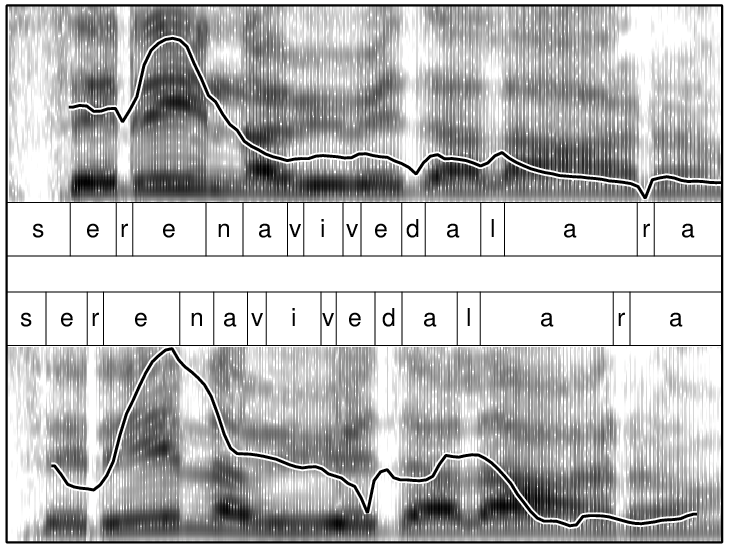
\includegraphics{images/401.png}}
\caption{Spectrogram, \textit{f0} track and phone segmentation for the sentence \textit{Serena vive da Lara} uttered with subject narrow focus, as a statement (top panel) and as a question (bottom panel).}
\label{fig401}\end{figure}

\subsubsection{Recordings}\label{sec4213}
Recordings of both corpora were made in the sound-treated booth\footnote{We would like to thank Elio Marciano for allowing us to use the facilities at \textit{CIRASS} (Centro Interdipartimentale di Ricerca per l'Analisi e la Sintesi dei Segnali), Naples University ``Federico II'', and Giovanni Abete for his assistance.}. Speakers were recruited among 20-25 years old students of the School of Humanities; they were all native speakers of the Neapolitan variety of Italian. The trials were prompted on a computer screen using \textit{Perceval} \citep{andre2003perceval}, while the recordings were made using an AKG MicroMic C520 head-mounted microphone linked through a Shure X2u adapter to a personal computer running \textit{Audacity} \citep{audacity2006audacity}. 

For the \textit{Orlando} corpus, 30 speakers read 3 repetitions of the 6 interpretations for each of the 3 test sentences, for a total of 1620 items. For the \textit{Danser} corpus, 21 speakers read 3 repetitions of the 6 interpretations for each of the 2 test sentences, for a total of 756 utterances. Each experimental item was isolated from the recording blocks and opportunely coded using a scripted procedure in \textit{Praat} \citep{boersma2008praat}. A small amount (ca. 3\%) of the recorded utterances contained disfluencies or prosodic breaks after the focussed constituent, and were thus excluded from analysis. 

\subsection{Forced alignment}\label{sec422}
The 2376 utterances from the two corpora were segmented to phones. Since every sentence was composed by eight CV syllables, phone segmentation would have required the placement of more than 35000 segmental boundaries, making manual segmentation extremely costly. We opted for an automated segmentation procedure, based on forced alignment. In the absence of free forced alignment tools for Italian (but now see \citealt{bigi2012speech}), we decided to create our own tool, \textit{ASSI} (Automatic Speech Segmentation for Italian; see \citealt{cangemi2011automatic}). The tool requires as input (1) sound files, (2) orthographic transcriptions and (3) lexicon with pronunciation variants; it yields as output a \textit{Praat}-compatible segmentation file. Data from our corpora are especially suited for use with \textit{ASSI}: by providing an orthographic transcription of 5 sentences and a phonological transcription of 12 words, we obtained a segmentation for 2376 utterances in 38016 phones. In order to maximize performances, test sentences were designed such as to avoid the use of phonemes which were scarcely represented in the corpus used to train the acoustic models (viz. the \textit{CLIPS} corpus, \citealt{savy2009clips}). 

The quality of the output was scrupulously tested (see \citealt{cangemi2011automatic} for details). Testing involved comparisons with manual expert segmentation of both boundary placement and of metrics extracted from the segmentations. As for boundary placement, 94\% of the markers placed by \textit{ASSI} are within 20 ms from the manual reference in both a subset of the \textit{Orlando} corpus (405 boundaries) and  of the \textit{APASCI} corpus (17474 boundaries; see \citealt{angelini1993baseline}). If error from the reference is extended to 30 ms, \textit{ASSI} performances reach 97\% with \textit{APASCI} and 99\% with the \textit{Orlando} corpus. More importantly for our purposes, \textit{ASSI} and manual segmentations for 27 utterances with three different focus patterns in the Orlando corpus were used to calculate Local Phone Rate curves (see Section~\ref{sec442}). The obtained functions were compared pairwise for focus condition using a two sample F-test for equal variances, and no significant difference was found.

\section{Experiment 1}\label{sec43}
As we saw in the introduction of this chapter, tempo has been related to sentence modality contrasts only in recent studies. Durational differences in question/statement contrast have been reported for various languages, on the basis of material drawn from differently designed corpora and measured at different degrees of precision. Two working hypotheses seem to have informed, more or less implicitly, the studies on this topic: first, that there are durational differences across statements and questions, and second, that these differences are localized in specific portions of the utterance. Experiment 1 was devised in order to test an explicitly operationalized version of these two hypothesis (Section~\ref{sec431}), by capitalizing on the mixed results available from the literature that we review in this section.

In order to illustrate the issues in comparability and compatibility of the studies in the literature, we group the available results in Table~\ref{tab41}. For each study (column 1) we indicate the investigated language(s) (column 2) and which modality is associated with longer durations (or slower speech rates) at the \textit{utt}erance level (column 3)\footnote{We use \textit{S} for statements, \textit{Q} for questions and \textit{=} for statistically non-significant differences. Cells are left empty if no relevant results are available.}. 

As Table~\ref{tab41} shows, questions and statements do display different global durations at the utterance level for a variety of languages. However, no universal trend can be extracted from the data: questions are longer in some languages and shorter in others, thus the effect of sentence modality on tempo is language-specific. More interestingly, as the comparison from data on NI shows, the available studies report opposite results even for the same regional variety of a given language: according to \citet[table 6]{maturi1988intonazione}, sentences are slightly shorter when uttered as a question, but the reverse is true for \citet[p. 163]{petrone2008role}\footnote{Approximatively, the magnitude of the effect is 30 ms for 1-second long utterances for Maturi and 70 ms for 1.4-second long utterances for Petrone.}. 

\begin{landscape}
\begin{table}[p]
\centering
%\resizebox{\linewidth}{!} { PUT TABULAR HERE }
\begin{tabular}{c c c c c c c c}
Reference & Language & Utt & Beg & End & Syntax & Focus & Domain \\
\hline\hline
Maturi & Neapolitan & S & & & (S)V(O) & ? & Utterance\\
1988 & Italian & & & & & & \\
\hline
Ryalls et & Canadian & S & & Q & & & Final \\
alii 1994 & French & & & & & & syllable \\
\hline
Smith & Hexagonal & & & = & & & Final \\
2002 & French & & & & & & vowel \\
\hline
Rialland & Various & Q & & Q & & & Final \\
2004 & African & & & & & & vowel \\
\hline
van Heuven & Manado & S & & S & & & Foot \\
\& & Malay & & & & & & \\
van Zanten & Dutch & S & = & = & SOV & & Interstress \\
2005 & & & & & & & stretch \\
\hline
Petrone & Neapolitan & Q & S/Q & Q/? & SVO & O & Phonological \\
2008 & Italian & & & & & & word \\
\hline
De Dominicis & Bomarzo & Q & & & & & Foot \\
2010 & (Italy) & & & & & & \\
\end{tabular}
\caption{Synopsis of findings in the literature on tempo and sentence modality}
\label{tab41}\end{table}
\end{landscape}

However, a closer examination of the test items shows that other factors should be taken into account when comparing these results, such as syntax and information structure (see respectively columns 6 and 7): whereas Petrone only used SVO sentences with narrow focus on the Object, the sentences used by Maturi are syntactically different (SV, VO and SVO, with no indication of information structure). Tempo variations are not only language-specific, but they also seem to depend on factors other than sentence modality. 

An additional layer of variability is represented by speaker-specific behaviour, which can turn into an interpretative problem given the usually low number of subjects (often between two and ten). For instance, the two NI speakers in Petrone's corpus have opposite patterns as for the first phonological word of the utterances (column 4). This brings us to another source of complication in the results: other studies as well have tried to individuate more specifically the domain of durational differences across sentence modalities, but the global picture is even more complicate to seize since the domains are of different size (column 8)\footnote{For this reason, columns 4 and 5 only broadly refer to ``Utterance \textit{beg}inning'' and ``Utterance \textit{end}''.}. Specifically, \citet{smith2002prosodic} focuses on the last vowel, \citet{ryalls1994effects} on the last syllable, \citet{vanheuven2005speech} on the last foot (Manado Malay), \citet{petrone2008role} on the first and last phonological word, and \citet{vanheuven2005speech} on ``the stretch between the stressed syllable on the subject and that on the object'' (Dutch). 

In sum, we can draw three main conclusions on the methodological level from the literature synopsis. First, it is clear that a tight control of the test material is needed: since syntactic and information structure can affect the results (as data on NI shows), the experimental design must be tailored accordingly. For this reason, in our corpora we only used SVO sentences and we varied orthogonally the position of focus\footnote{Focus will be actually treated as a \textit{factor} in E2.}. Second, data from Petrone also shows the possibility of strong inter-speaker variability: for this reason, our corpora include recordings from more than fifty speakers altogether. Third, accurate comparisons as for the precise localization of durational differences are made impossible by the use of different metrics across the various studies. Measuring the entire utterance duration alone, for example, would reduce the possibility of comparing specific results at, say, the syllable level. For this reason, even if a thorough comparison with the other studies is not our priority, we measured the duration of individual segments, thus permitting their grouping in higher level structure of all sizes.

\subsection{Hypotheses}\label{sec431}
The literature synopsis also enables an explicit elaboration of the research hypotheses which implicitly underlie previous work. In general terms, it appears that sentence modality has a \textit{global} effect on tempo, namely at the utterance level, though in opposite ways across languages (questions are shorter in Manado Malay, Orkney English and Dutch, but longer in various African languages, in Bomarzo's dialect and in NI). Morerover, sentence modality also seems to have a \textit{local} effect on tempo, in that durational differences are more intense on some specific portions of the utterance (though with conspicuous differences across studies and languages, e.g. from the first phonological word to the last vowel). Given the mixed results in the literature, the two hypotheses are operationalized in the most general terms possible: 

\begin{description}
   \item[H1] \textit{sentences have a different duration when uttered as questions or statements}, independent of the direction of the  effect. Utterance length (U) is different for questions (Q) and statements (S):\\ $U_{Q} \neq U_{S}$.
   \item[H2] \textit{durational differences are localized in some specific portions of the utterance}, independent of their position and their size. Duration of the various (from 1st to nth) segments (P) in a question (Q) is not a linear transformation or uniform stretching/compression (a) of duration in the respective statement (S):\\ $P\{1,n\}_{Q} \neq aP\{1,n\}_{S}$.
\end{description}

Note that the validation of H1 is not a necessary prerequisite for the existence of different durational patterns across the utterance. This is because we cannot exclude a priori the possibility of generating the same utterance duration from two different (but counter-balanced) durational patterns at the segment level. Thus, H1 and H2 can be combined to test whether sentence modality affects tempo at a global (utterance) or at a local (here, segment) level (see Table~\ref{tab42}).

\begin{table}[h]
\centering
%\resizebox{\linewidth}{!} { PUT TABULAR HERE }
\begin{tabular}{c c | c c}
Hypothesis & & \multicolumn{2}{c}{H2}\\
& Confirmed & No & Yes\\
\hline
\multirow{2}{*}{H1} & No & NO & LOCAL\\
 & Yes & GLOBAL & GLOBAL+LOCAL\\
\end{tabular}
\caption{Summary of hypotheses}
\label{tab42}\end{table}

Should H1 and H2 be disconfirmed, we would have evidence of a total absence of sentence modality effect on tempo patterns (H0). If H1 is confirmed and H2 is disconfirmed, we could conclude that modality affects utterance duration as a whole. In case H1 is disconfirmed and H2 confirmed, we would have evidence of local tempo variations which do not affect total utterance duration (i.e. they would be counterbalanced). Should both H1 and H2 be confirmed, we could conclude that modality affects in the first place some specific portions of the utterance, and that this effect is visible in terms of total utterance duration as well. 

\subsection{Method}\label{sec432}
We evaluated these two hypotheses using data from both corpora and extracted with scripted procedures in \textit{Praat}. For the validation of H1, no measurement other than utterance duration was needed. As for H2, we extracted individual phone durations and coded them using the ordinal number of parent syllable preceded by an identifier for consonant or vowel (e.g. segment [i] in sentence (3) was coded as phone position V2; see  Figure~\ref{fig402}). Phone durations were normalized on parent utterance duration in order to account for idiolectal variations in speech rate. This normalization has the effect of blurring eventual global differences among sentences uttered as questions or statements as well; however, since H1 and H2 are evaluated independently, no confound is possible. Indeed, it permits an immediate qualitative evaluation of H2 given a plot of relative duration against phone position: for any given value of \textit{a} (see Section~\ref{sec431}), H2 is validated by completely overlapping polylines. 

Statistical tests will be described separately for the two hypotheses in the next section, with respect to data from the \textit{Danser} corpus.

\subsection{Results}\label{sec433}

Hypothesis 1 was tested with a linear mixed model which predicted the dependent variable \textit{Utterance Duration} by using the fixed factors \textit{Modality} (question or statement), \textit{Focus} (on NP, VP or PP) and \textit{Sentence} (two levels, see (3) and (4)), adding a random intercept for the 21 Speakers. Both the factor \textit{Modality} and its interactions with the factor \textit{Focus} did not reach significance ($t<2$), leading to the rejection of H1. A Likelihood Ratio Test comparing the model with the fixed factors \textit{Focus} and \textit{Sentence} (and their interaction) with a model including \textit{Modality} as well showed no significant differences ($\chi^{2}=9.9, df=6, p=0.13$). 

For the sake of completeness (see footnote 4), we report that the factor \textit{Focus} on its own did reach significance ($|t|>3$), indicating that, compared to NP-focused utterances, VP-focused utterances are longer while PP-focused utterances are shorter (mean difference of about $\pm$30 ms on a mean duration of 1.15 s).

We then tested H2 by running a linear mixed model predicting \textit{Phone Duration} from three fixed factors: \textit{Focus} (three levels: NP, VP and PP), \textit{Sentence} (two levels) and the \textit{Combination} of Phone position (from C1 to V8) and Modality (Question or Statement).  A successive difference contrast was associated to the 32 levels of the factor \textit{Combination} in order to verify which phone position yielded significantly different durational values across modality. 11376 phone durations were analyzed, and a random intercept was added to account for variability across the 21 Speakers. A Likelihood Ratio Test showed that, compared with the model including three-way interactions, a two-way interactions model had a slightly (and significantly) smaller Likelihood, but better AIC and BIC. Consequently, in what follows we will only refer to the more economical model. 

\begin{figure}
\centering
\resizebox{\linewidth}{!}{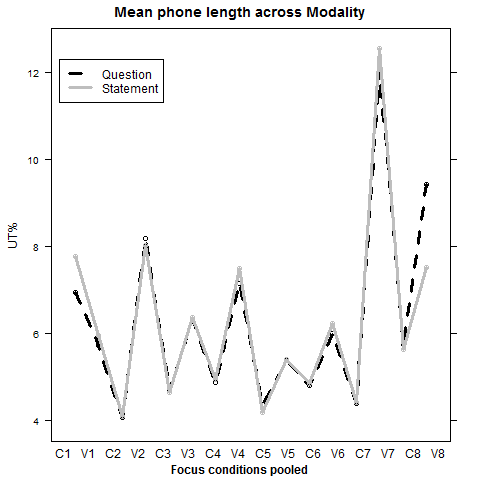
\includegraphics{images/402.png}}
\caption{Phone duration against position (E1, H2).}
\label{fig402}\end{figure}

Our model showed a number of significant contrasts, but since their combined size effect was less than 10 ms (see \citealt{lehiste1970suprasegmentals} for a discussion of difference limina in the perception of duration for speech signals), they will not be further commented here. Apart from that, three significant interaction coefficients between \textit{Combinations} and \textit{Focus} were found, indicating (together with the non-interacting contrasts) that the stressed vowel of a focused phrase is significantly longer ($ \sim $10 ms) in Statements. Most importantly, independently of other factors, the two most highly significant contrasts ($pMCMC<0.001$) indicated that the first segment (C1) is longer ($ \sim $12 ms) in Statements and the last segment (V8) is longer ($ \sim $20 ms) in Questions.

A more readable account of these results can be provided by plotting, for every phone, its \textit{Position} in the utterance (x-axis) against its \textit{Duration} (normalized on utterance length, y-axis) for the two levels of the factor \textit{Modality} (question, dashed black line, and statement, continuous grey line; see Figure~\ref{fig402}). If \textit{Modality} were not significant, we would expect two exactly overlapping polylines, but the plot does show localized differences (mainly on C1 and V8), thus confirming H2.

\subsection{Discussion}\label{sec434}
Our results show that sentence modality does not affect the duration of the entire utterance, disconfirming H1, but that it affects individual phone durations, thus confirming H2. As a result, E1 found support for the existence of a \textit{local} effect of sentence modality on tempo (see Table~\ref{tab42}). Specifically, the first segment is longer in statements and the last is longer in questions, but total duration is not significantly different. These findings are not immediately compatible with results available from the literature. In this section, we provide some elements which could account for the difficulties in drawing a coherent picture from the available studies. 

The first unexpected result is the absence of durational differences at the utterance level for the two modalities. Indeed, speculating on the results available at the time, \citet{vanheuven2005speech} even suggested that questions might have been universally linked to a faster speech rate (and thus to shorter durations). We will come back in greater detail to this issue at Section~\ref{sec451}: for the moment it suffices to say that, together with other studies in the literature, our data is rather consistent with a language-specific nature of the eventual temporal encoding of sentence modalities. This is perhaps the main factor accounting for the great variance in results in the literature.

On the other hand, our results are in line with the literature in showing that durational differences might be concentrated at specific portions of the utterance. However, because of the choice of different levels of analysis and measurement among the various studies, no direct comparison is possible. It is nonetheless striking that durational differences seem more robust at utterance ends in nearly all the studies which reported a localized effect. Our results seem to confirm this trend, showing that the first segment is longer in statements and the last segment is longer in questions. Since phone duration is inversely correlated with speech rate, we can reformulate this finding by saying that sentences are faster in their initial portion when uttered as questions and faster in their final portion when uttered as statements. That is, if we take speech rate to be variable in time, we might expect it to accelerate in statements and decelerate in questions. We will try to use such a dynamic metric in E2; for the sake of our present discussion, the main finding is that the use of excessively synthetic metrics (such as total utterance duration alone, as in the case of \citealt{maturi1988intonazione}) could hinder the evaluation of localized effects.

Our last observation concerns the role of syntactic and information structure. Previous studies based on reading tasks featured no balancing of focus placement, and in some cases different syntactic structures as well. In our study, each sentence had the same syntactic structure made of three positions, and was uttered in all of the three possible narrow focus patterns. Our results show that shifting focus placement can indeed affect both utterance and phone durations. A closer investigation of focus placement as a factor will be provided by E2, but for the purposes of our present discussion we can at least state that differences in syntactic and information structure can be regarded as the third element accounting for the mixed results in the literature on tempo and modality.

\section{Experiment 2}\label{sec44}
In E1 we gathered evidence for a localized effect of sentence modality and information structure on tempo, pointing to the need for (1) accurate metrics in measuring durational differences and (2) control for focus. Experiment 2 elaborates on these two points, respectively by providing an alternative visualization of durational data based on a continuous metric and by testing the effect of focus on temporal patterns.

As for the first point, we have seen that temporal differences across questions and statements are localized within the utterance, yet they counterbalance each other at a global level. This means that our data is best represented using a metric which computes and displays durational patterns in an inherently relational way. In the discussion of data on phone durations (see Section~\ref{sec434}), we have already suggested that differences in the duration of the segments at utterance ends could be seen as the result of speech rate variations in time. Instead of calculating a single value for the speech rate of the entire utterance, we could calculate several values using a sliding window on the segmented signal, thus obtaining a continuous representation of speech rate variations. In this way, the differences between questions (which have shorter initial segments and longer final segments) and questions (which have longer initial segments and shorter final segments) could be seen, more synthetically, as a difference between globally decelerating and accelerating speech rate across the utterance. In this way, local differences in phone durations but global equality of utterance duration would both stem from a single propriety. The details of the algorithm for the calculation of continuous speech rate data will be presented at Section~\ref{sec442}.

The other main finding of E1 was that information structure must be controlled for in order to gather reliable data on temporal patterns. The sentences used in E1 were designed such as to be elicited in a variety of focus placement conditions; focus placement was controlled (and balanced) under the assumption that it has an effect on temporal patterns. This assumption is motivated by the fact that, in Italian, focalization entails accenting and thus lengthening \citep{farnetani1990rhytmic}. Experiment 2, however, turns this assumption into an hypothesis, thus transforming focalization from a controlled (E1) to an independently manipulated (E2) factor. In particular, with respect to the intricacies of the results available in the literature, our interest lies in the possibility that sentence modality and focus structure interact in such a way that surface differences in temporal patterns could be blurred.

\subsection{Hypotheses}\label{sec441}
We know that the temporal structure is affected both by focus placement (through accenting and consequent lengthening phenomena) and sentence modality, but do these two factors operate in a completely independent way? We operationalized this hypothesis by predicting that, if focus and modality were independent, the overall modality-induced differences (faster utterance beginning and slower utterance ending for questions) should be found regardless of focus condition. 

Unlike the other experiments in this book, the evaluation of this particular hypothesis will be based on qualitative observations. This choice is not only motivated by the relative rareness of statistical analyses of continuous data in linguistics (but see recent work on Functional Data Analysis, e.g. \citealt{gubian2010automatic}), but also by the necessity of evaluating the visual impact of the proposed metric. 

\subsection{Method}\label{sec442}
Using the ASSI phone segmentation as input, we extracted a continuous representation of speech rate variations by using a slightly modified version of the Local Phone Rate (henceforth \textit{LPR}) function proposed by \citet{pfitzinger2001phonetische}. As indicated by its name, LPR is calculated for a given point in time by counting the number of phone boundaries falling inside a window centred around the point itself. If LPR is calculated for multiple points and plotted against time, the result is a graphical display of variations in speech rate as a function of time. Of course, the calculation relies on a number of parameters which have to be adapted to the characteristic of the speech material under examination. In particular, the size of the analysis window and of the steps must be short enough to capture variations of the desired magnitude. In our case, we decided to use a 0.2s window and 0.01s steps.

We also modified the original formula in two respects. First, we calculated no values when the window exceeded the signal boundary. That is, given an analysis window 0.2s long, we calculated no LPR values for $t<0.1$ and $t>T-0.1$ ($T$ being total utterance duration). Moreover, the original formula was meant to deal with speech material containing pauses as well. Since utterances with pauses and disfluencies were excluded from our corpora, we could simplify the original formula in this respect. As a result, LPR was calculated using the formula in (5), through the use of an automated procedure in \textit{R} \citep{r2008r}:

\begin{description}
   \item[(5)] $LPR_{i}=\frac{\frac{t_{(l+1)}-(i-\frac{w}{2})}{t_{(l+1)}-t_{l}}+\frac{(i+\frac{w}{2})-t_{r}}{t_{(r+1)}-t_{r}}+r-l-1}{w}$
\end{description}

In the formula, $w$ stands for the analysis window length and $i$ for the analysis point in normalized time, ranging in its actual values from $w/2$ to $T-w/2$. The number of phones entirely encompassed before the right and left window boundary are indicated respectively with $r$ an $l$; given the phone $x$, the following phone is indicated as $x+1$. The point in time where the boundary for phone $x$ falls is indicated with $t_{x}$. Figure~\ref{fig403} shows two examples of LPR calculation.

\begin{figure}
\centering
\resizebox{0.88\linewidth}{!}{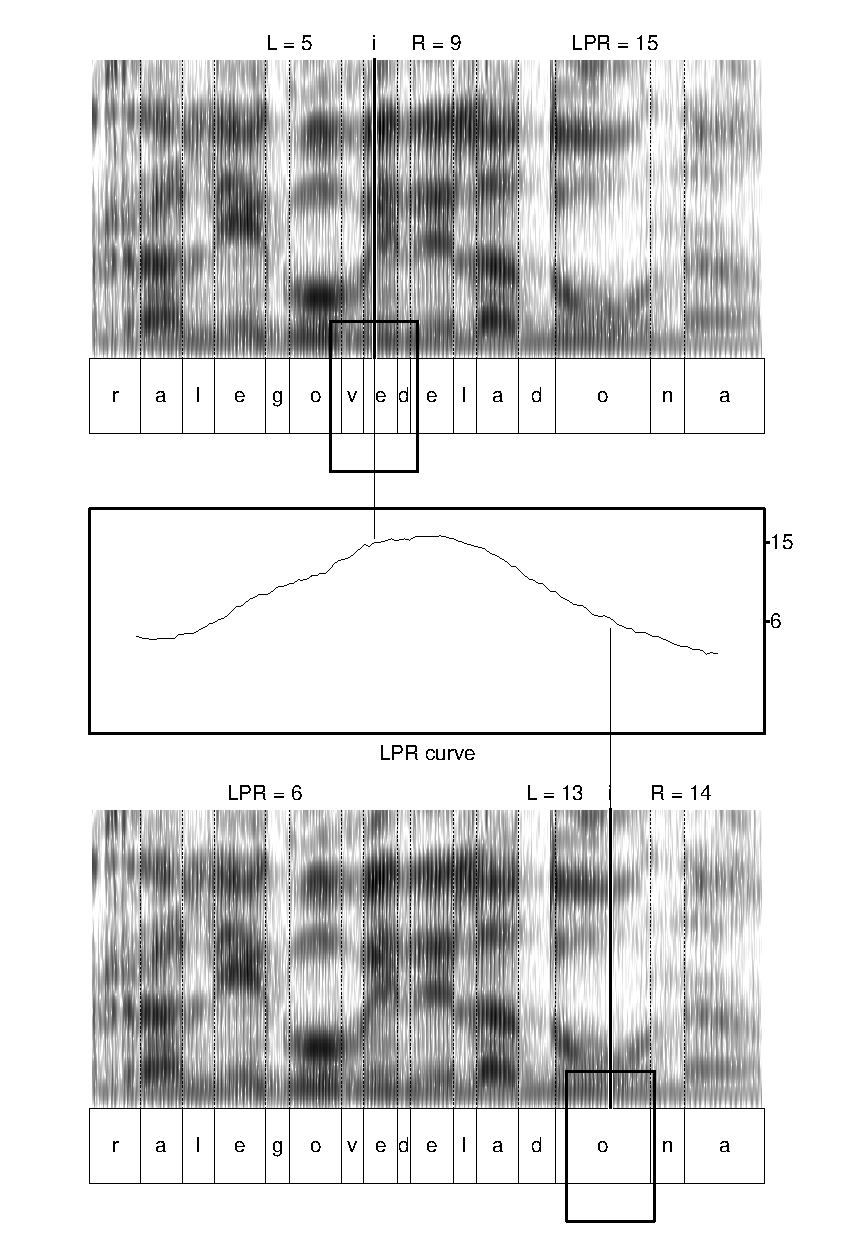
\includegraphics{images/403.pdf}}
\caption{LPR calculation for the sentence \textit{Ralego vede Ladona} uttered as an object-focus question.}
\label{fig403}\end{figure}

In short, for each point in the normalized time of the utterance, we calculated the Local Phone Rate as the number of phones falling inside a window centred on the time point, weighting accordingly the phones partially included in the window, and dividing the total by the size of the window. LPRs extracted for individual utterances were averaged across speakers and utterance repetition within modality and focalization conditions, and plotted against normalized time.

\subsection{Results}\label{sec443}
Since none of the previous studies featured Verb-focussed test items, and since the discrete analysis found durational differences at the periphery of utterances (while verbs occupy their medial position), in what follows we will concentrate on Subject- and Object-focussed utterances.

Data from the \textit{Orlando} corpus shows that LPR curves for S-focussed utterances conform to results from the discrete analysis (see Section~\ref{sec433}) and provide a readable display of modality induced effects: questions are characterized by a faster speech rate at their beginning and a slower speech rate at their end, while the opposite is true for statements, which accelerate through the utterance (see Figure~\ref{fig404}, left panel). Results for O-focussed utterances, show indistinguishable LPR curves for question and statements (see Figure~\ref{fig404}, right panel). 

\begin{figure}
\centering
\resizebox{\linewidth}{!}{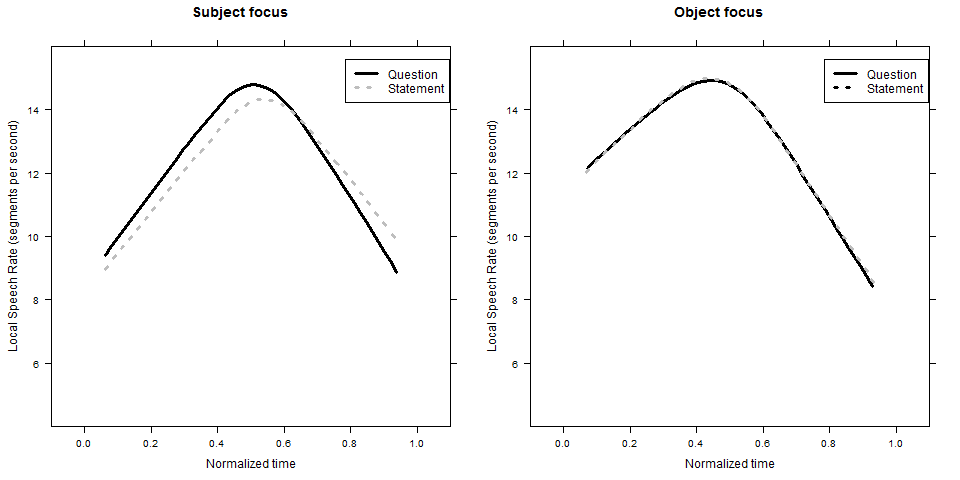
\includegraphics{images/404.png}}
\caption{Local phone rate against normalized time (E2).}
\label{fig404}\end{figure}

\subsection{Discussion}\label{sec444}
Visual inspection of the LPR curve sets provides a qualitative validation of our research hypothesis on the interaction between Modality and Focus. The null hypothesis of equal differences between questions and statements independent of focalization was not verified. The finding of exactly matching LPR curves for O-focussed utterance, however, is particularly interesting, and deserves further elaboration.

\subsubsection{Post-hoc analysis}\label{sec4441}
A possible explanation for this result lies in one of the minor findings of E1. The discrete analysis found significant interactions between Modality and Focus, indicating that the stressed vowel of a focussed phrase is significantly longer ($ \sim $10 ms) in Statements (see Section~\ref{sec433}). This means that if the focussed phrase is at the beginning of the utterance (where Statements have slower speech rate), the difference will be even more salient. But if the focussed phrase is at the end of the utterance, where Questions have slower speech rate, the result could be the blurring of modality induced effects (see next section).

Another explanation for the different results from S- and O-focussed items comes from a possible flaw in corpus design. As we said above (see examples (1-2) at Section~\ref{sec421}), Statement interpretations were elicited by presenting the test items along with a context paragraph requiring correction from speakers. In Statement condition, test items were recorded along with a ``No'' which introduced the correction. The negation was then excised from the final test item. In the striking majority of cases, the negation and the test item were uttered as two separate intonational phrases, with a strong phrase break and a silent pause between the two. However, in some cases negation and test item were uttered as a single intonational phrase, a fact which could affect segmental durations. Crucially, utterances with a single intonation phrase were more frequent for O-focussed interpretations. We then decided to plot separately utterances with one and two intonational phrases from the \textit{Danser} corpus. Utterances were assigned to one of the two classes not only by accurate listening, but also by visual inspection of intensity profiles, under the conservative assumption that while prosodic breaks do not necessarily entail silences, silences do cue prosodic breaks. Figure~\ref{fig405} shows a plot of intensity profiles in a window centred around the end of the negation, for all statement utterances from a given speaker. Dips in the intensity contour were taken as a cue to separate phrasing; for this speaker, thus, only two utterances (RS1B3 and RS3A1) had no phrase break after the negation.

\begin{figure}[!htbp]
\centering
\resizebox{\linewidth}{!}{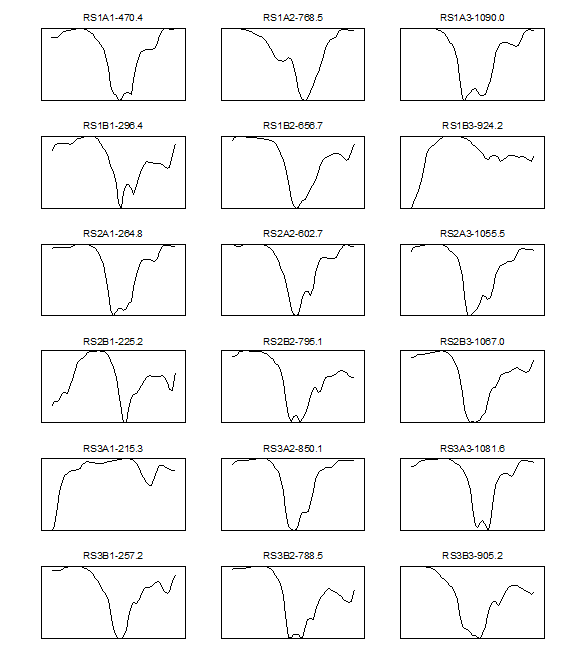
\includegraphics{images/405.png}}
\caption{Intensity contours centered around stimulus onset.}
\label{fig405}\end{figure}

If we exclude single phrased utterances from comparison with questions, durational differences between questions and statements for S-focused items are even more visible (compare dashed grey line with dot-dashed black line in Figure~\ref{fig406}, left panel). Again, statements are slower in the beginning, and questions are slower towards the end. As for O-focused items, we see that statements are comparable to questions in the end portion of the utterance, but they are slower in the beginning. 

\begin{figure}[!htbp]
\centering
\resizebox{\linewidth}{!}{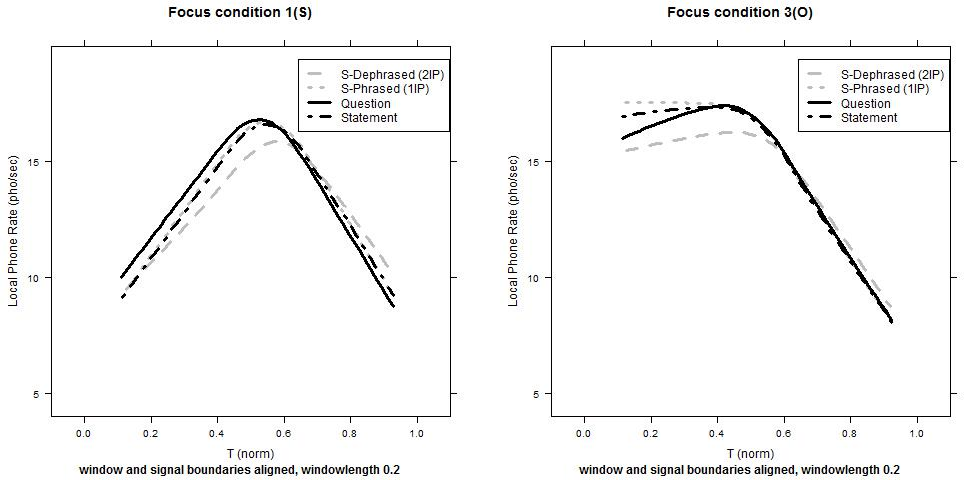
\includegraphics{images/406.png}}
\caption{Local phone rate for stimuli with different phrasing.}
\label{fig406}\end{figure}

\subsubsection{Interpretation of results}\label{sec4442}
To summarize, the analysis of LPR curves on comparably phrased utterances in the Danser corpus showed that sentence modality and focus interact in determining speech rate patterns. Specifically, S-focus utterances begin faster in questions while ending faster in statements. As for O-focused utterances, questions have faster beginnings. Our results can be neatly accommodated in a superpositional account of speech rate determination, according to which variations in speech rate patterns are determined by modality, by focus, and by their interactions\footnote{An exhaustive model of tempo management is clearly beyond the scope of this chapter. The account we present in this section is merely meant to provide a first structuring of the available data, and no claims are made on the mechanisms which shape speech rate patterns. Even the ``generative vibe'' of this account, evoking underlying patterns which are modified by intervening factors down to a final output, is only meant as an expository device. See Section~\ref{sec45} for discussion on the possible linguistic reality of the interaction between Focus and Modality.}. 

First of all, as both Figure~\ref{fig404} and~\ref{fig406} show despite the particular details, Focus has a direct effect on speech rate in that speech rate is slower on focussed constituents. For example, given SVO sentences, the first part of the utterance is faster if S bears no focal accent: see higher LPR values for O-focussed utterances in the first third of the curves\footnote{The effect does not seem to be symmetrical, in that we do not find the same difference between focussed and unfocussed Objects, indicating that speech rate at utterance end might be affected by other factors (such as preboundary lengthening, for example). Our corpora were not designed to test this claim, so results from sentences with syntactic structures other than SVO are needed in order to settle this issue.}. Figure~\ref{fig406} also shows that speech rate in statements is lower at the beginning of the utterance for both S- and O-focussed items. This could be ascribed to a modality-related effect, slowing down statements in their beginning, as discussed in the presentation of results from the discrete analysis (see Section~\ref{sec434}). The discrete analysis also showed that questions tend to be slower towards the end of the utterance. This is confirmed by our continuous display only for S-focussed utterances. O-focussed utterances have a comparable speech rate at utterance end in both sentence modalities. However, this is where the Focus-Modality interaction might play its role. As we said above (Section~\ref{sec433}), stressed vowels are longer in focussed constituents than in non focussed constituents, but they are yet longer in focussed constituents in statements. This interaction between focus and modality could be responsible for enhancing speech rate differences in the first portion of S-focussed utterances (where statements are yet slower than questions) and by counteracting them in the last portion of O-focussed utterances (yielding comparable speech rate values). 

Table~\ref{tab43} shows, separately for utterances focussed on the Subject or the Object (first row), which portion of the utterance (``S'', Subject at utterance beginning, and ``O'', Object at utterance end) is expected to be lengthened (``+'') according to Focus induced effects, Modality induced effects, and to their interaction (first column) in the two modalities (second row).

\begin{table}[h]
\centering
%\resizebox{\linewidth}{!} { PUT TABULAR HERE }
\begin{tabular}{c || c c | c c || c c | c c}
& \multicolumn{4}{c}{Subject-focus} & \multicolumn{4}{c}{Object-focus}\\
& \multicolumn{2}{c}{Statement} & \multicolumn{2}{c}{Question} & \multicolumn{2}{c}{Statement} & \multicolumn{2}{c}{Question}\\
& S & O & S & O & S & O & S & O\\
\hline
Focus & + &   & + &   &   & + &   & + \\
Modality & + &   &   & + & + &   &   & + \\
Interaction & + &   &   &   &   & + &   &  \\
\hline
& +++ & & + & + & + & ++ & & ++ \\
\end{tabular}
\caption{Overlay model}
\label{tab43}\end{table}

According to the table, in the S-focus condition we expect statements to be slower at the beginning and questions to be slower at the end of the utterance; in the O-focus condition, we expect statements to be slower at the beginning but no difference at the end of the utterance. A comparison with actual data (see Figure~\ref{fig406}) yields a very good match.

\section{General discussion}\label{sec45}
Evidence from E1 and E2 shows that sentences have different durational patterns when uttered as questions or statements. However, sentence modality does not affect utterance duration as a whole, but rather particular portions of the utterance. Specifically, compared to questions, statements are faster (shorter phone durations) at the beginning and slower (longer phone durations) towards the end. Moreover, differences in durational patterns across questions and statements are not independent of focal accent placement, up to the point that speech rate differences can be reduced or blurred in some circumstances (as in Object-focussed SVO sentences). 

These findings account for the difficulty in drawing a clear picture from the various studies in the literature, which analyse durational patterns for different languages at different degrees of finesse, and do not always control for focus placement or syntactic structure. They also enable an examination of the allegedly universal character of the link between questions and fast speech rate (see Section~\ref{sec451}). And, more importantly for the general purposes of our thesis, they question the degree of phonetic information that can or must be included in prosodic abstract categories (see Section~\ref{sec452}).

\subsection{Universality and specificity}\label{sec451}
The finding of no global effect of sentence modality on utterance duration, together with those emerging from the literature on the topic, argue in favour of language-specific relationships between tempo and sentence modality. An alternative view is embraced by \citet{vanheuven2005speech}. Cautiously speculating on their results on Dutch, English and Manado Malay, they suggested that the higher speech rate found in questions could be interpreted as a (trend to a) prosodic universal, based on both ethological, perceptual and production mechanisms. 

According to their account, faster speech rate could be taken as the temporal counterpart of high pitch values. From an ethological perspective, grammaticalization of high pitch as cue to question modality would be mediated by submissiveness \citep{ohala1984ethological,gussenhoven2004phonology}. Given that ``small (harmless) creatures have higher pitches, and make faster movements, than large (dangerous) creatures'' \citep[p. 97]{vanheuven2005speech}, faster speech rate could cue submissiveness as well. The link between higher pitch and faster speech rate would be testified by speech perception research as well: \citet{rietveld1987perceived} found that temporally unchanged utterances were judged by listeners to be faster when their pitch was artificially raised. As for production mechanisms, van Heuven and van Zanten build on \citeauthor{bolinger1964intonation}'s \citeyear{bolinger1964intonation,bolinger1989intonation} proposal that ``statements and questions are characterized universally by a dichotomy between relaxation (low, falling pitch) and tension (high, rising pitch), respectively'' \citep[\textit{ibid.}]{vanheuven2005speech}. If we take slower and higher speech rate to be correlates of relaxation and tension, we see how questions could be characterized by shorter durations. 

However, as pointed out by the authors themselves, the association between question on one hand and fast rate and high pitch on the other must be considered as ultimately arbitrary and conventional in the light of Rialland's findings on ``lax question prosody'' in some of the languages she surveyed (see the opening pages of this chapter for a more detailed review). Our results from E1 strongly support this arbitrary and language-specific account, since in our data questions do not seem to relate straightforwardly to a faster speech rate. Temporal patterns rather seem to interact in complicated ways with other linguistic dimension, such as syntactic and information structure, mediated through accent placement.

\subsection{Tempo (and intonation)}\label{sec452}
The interplay between modality and focus in shaping durational patterns is perhaps the major finding of E2. We suggested that differences in speech rate patterns between questions and statements across focus conditions can be framed in an additive model, where modality-induced effects are cumulated with focus-induced effects, and with their interactions as well. The modality-focus interaction also proved statistically significant and perceptually relevant in the analysis of discrete phone durations (see Section~\ref{sec433}), which showed that the stressed vowel of a focused phrase is longer in statements. 

In the perspective of research on prosodic detail, these differences are not interesting in themselves, as a simple quantitative account of phonetic facts. The main interest of the quantitative modality-focus interaction lies in the exploration of what we could call its linguistic reality. Can we really claim that speakers actually control individual segmental durations according to modality and focus options? More importantly, such a question relies on the implicit and unverified assumption that temporal aspects are \textit{independently} handled by speakers. In this view, tempo is indeed the formal dimension bridging post-lexical meaning with durational patterns (as we defined it in the opening pages of this chapter), and it constitutes along with intonation an orthogonal phonological axis to be included in the representation of prosody. To exemplify, in a rule-based text-to-speech system informed by this view we would expect to find, along with a low-level module responsible for the intrinsic pitch and duration adjustments, a prosodic module including both an intonational component (responsible for the generation of \textit{f0} contours) and a temporal component (responsible for the generation of durational patterns).

This view, however, is no more than a working hypothesis\footnote{Indeed, in the next chapter we will question it by exploring the perception of the durational differences we just reported on.}. The evidence we gathered in this chapter is actually rather consistent with the alternative view of a strong interplay between tempo and intonation. Indeed, what we called the modality-focus interaction in the quantitative account of the data is compatible with the view according to which prosodic categories are specified with respect to both the melodic and temporal dimensions. In AM terms, for example, we could imagine that a single paradigmatic option on the phonological level (say, a pitch accent) affects both the phonetic dimensions of fundamental frequency and duration. That is, the finding that stressed vowels in focussed phrases are longer in statements than in questions could be seen as due to a different pitch accent choice. In other words, pitch accents for narrow focus statements could be characterized not only by earlier peak alignment, but also by longer vowel durations\footnote{Informal tests based on the \textit{ShAli} corpus \citep{niebuhr2011shapers} yields results which are consistent with this claim.}. 

The exploration of this specific claim falls outside the scope of this chapter. What is crucial to the current discussion is that sentence modality does have an effect on segmental durations, independently of whether tempo should be regarded as orthogonal to or embedded into intonational contrasts. 

\section{Conclusion}\label{sec46}
In this chapter we documented the existence of produced temporal detail in read speech. Segmental durations in NI are affected not only by focus placement, but also by sentence modality. Specifically, while total utterance duration is not different across modalities, speech rate is faster at the beginning of the utterance for questions and at its end for statements. However, since stressed vowels of focussed constituents are longer in statements, modality-induced effect on durations can be blurred under some circumstances. These findings are not compatible with claims of a universal trend to faster speech rate in questions, and are instead consistent with language-specific behaviours. 

Differences in phone durations (or in speech rate) are not considered as cues to modality in the AM framework. As in the case of the consistently produced dynamic melodic detail we explored at Section~\ref{sec2}, it is possible that the current phonological categories accounting for sentence modality contrasts are phonetically underspecified. And, as in the case of the perception of dynamic melodic detail we explored at Section~\ref{sec3}, a perceptual validation will be instrumental in deciding whether these durational differences qualify as prosodic detail. The next chapter will thus focus on speech rate changes across utterances and the perception of sentence modality.

To conclude, the analysis of durational patterns across sentence modalities required the development and the fine-tuning of new and existing tools. The treatment of a great amount of data (more than 38.000 phone durations) was made possible by the development of \textit{ASSI}, a tool which performs forced alignment of Italian speech (see Section~\ref{sec422}) and which has been made publicly available\footnote{See http://www.esat.kuleuven.be/psi/spraak/demo/Italian/align.php . The scripts used for the calculation of Local Phone Rate curves are also available upon request.}. While being specifically developed for the purposes of this study, these tools could nonetheless prove useful for research on other topics, and represent along with the multiparametric resynthesis procedure (see Section~\ref{sec522}) an additional practical outcome of this work.